
\section{Application of CAN Protocol}

In this section,  the  project in  developing a prototype subsystem in a car that use CAN protocol as its communication standard will be discussed. For that, we use the problem as state in problem section as our main  reference for our prototype.

After we analyse the problem, we refine our requirement in requirement diagram as shown in ``Fig. \ref{fig:requirement_diagram}". As mentioned before, the protocol should work for long distance at high frequency.

\begin{figure}[h]
    \centering
    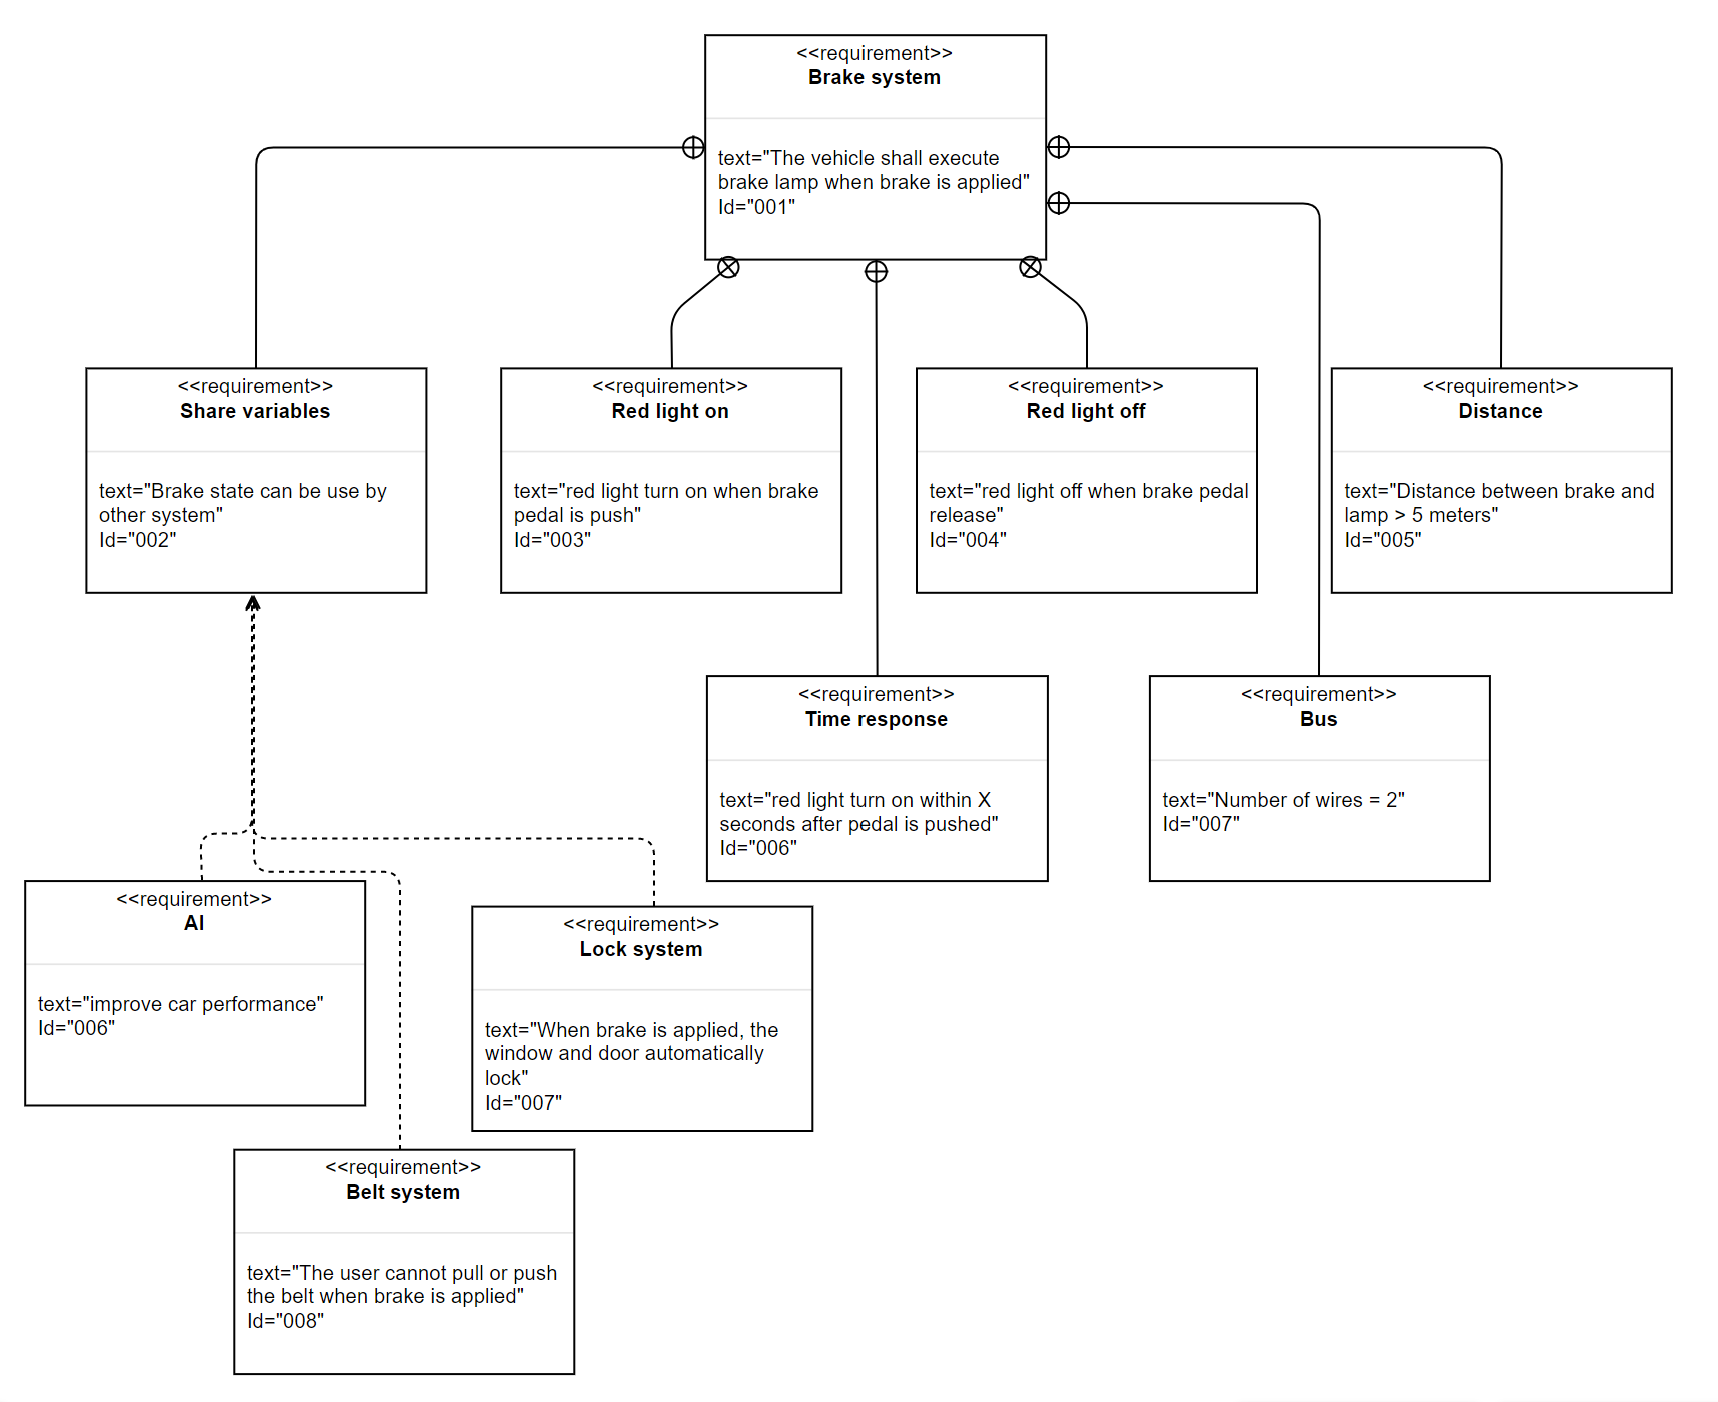
\includegraphics[width=0.5\textwidth]{requirement_diagram}
    \caption{Requirement Diagram}
    \label{fig:requirement_diagram}
\end{figure}

As explained in the problem section, Controller area network is chosen because it supports high data rate transfer for long distance and minimize number of wire used. Next, how the model of the solution will be explained based on the requirement.

\subsection{Application Model}

Our aim at this stage, which is modelling our solution, is to have a concrete system architecture including communication system where we will implement the communication protocol, so that it will be clear for us to do the implementation. The steps in this stage will be discussed in this section.

After analysing the scenario, requirements and protocol that we want to use, we create a use case diagram to have a clear boundary of the system as shown in ``Fig. \ref{fig:use_case_dagram}".

\begin{figure}[h]
    \centering
    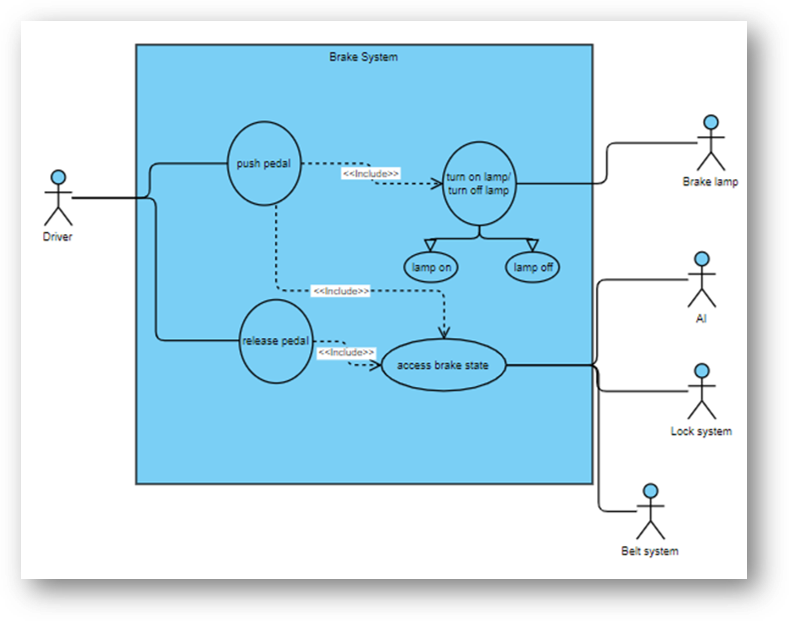
\includegraphics[width=0.5\textwidth]{use_case_dagram}
    \caption{Use Case Diagram}
    \label{fig:use_case_dagram}
\end{figure}

Next, we extend each use case using activity diagrams to understand their behaviour as pictured in ``Fig. \ref{fig:AD_pedalpush}", and  ``Fig. \ref{fig:AD_pedalrelease}". later we use all this diagram to make a sequence diagram to illustrate how object in the subsystem interact with each other as shown in ``Fig \ref{fig:sequence_diagram}".

\begin{figure}[h]
    \centering
    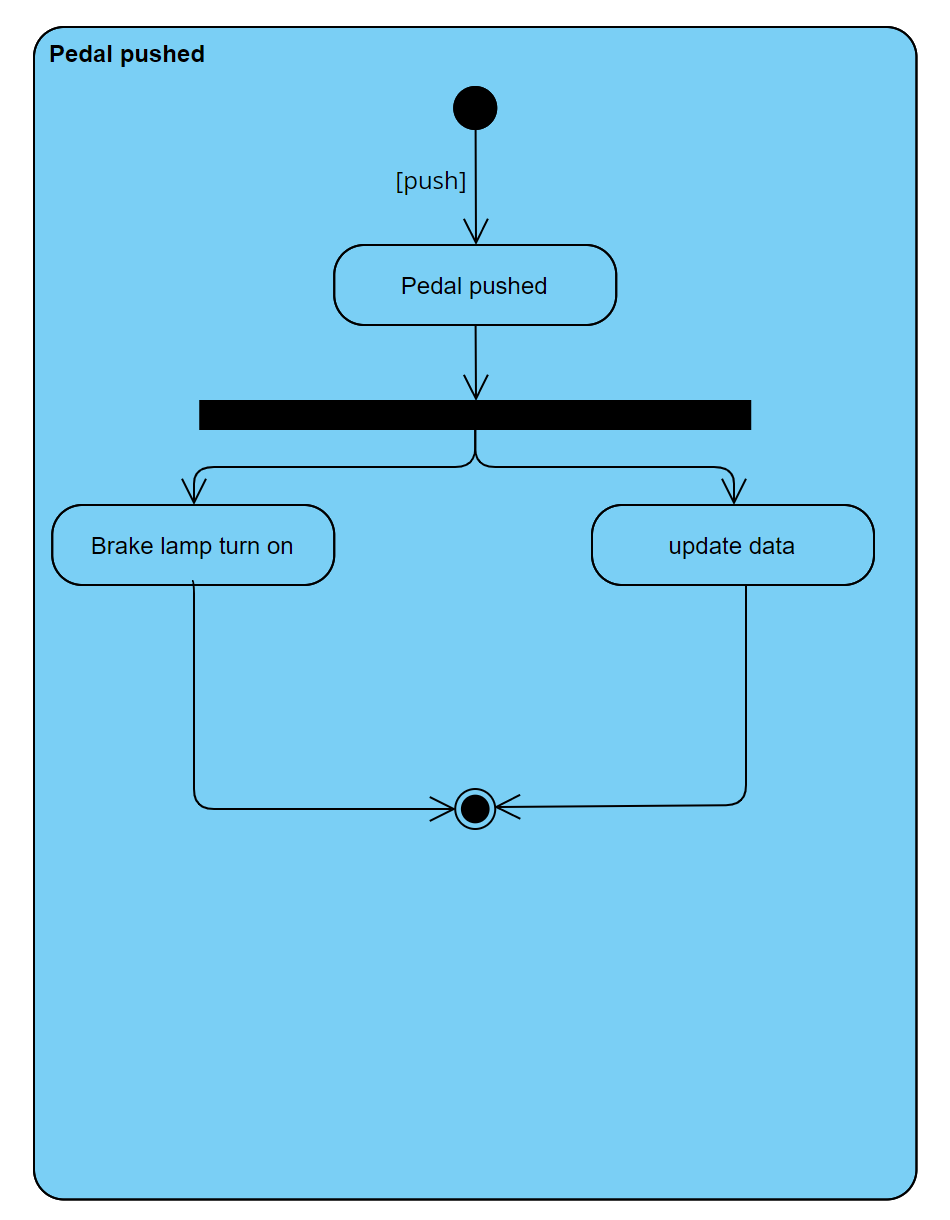
\includegraphics[width=0.3\textwidth]{AD_pedalpush}
    \caption{Activity diagram when the pedal pushed}
    \label{fig:AD_pedalpush}
\end{figure}
\begin{figure}[h]
    \centering
    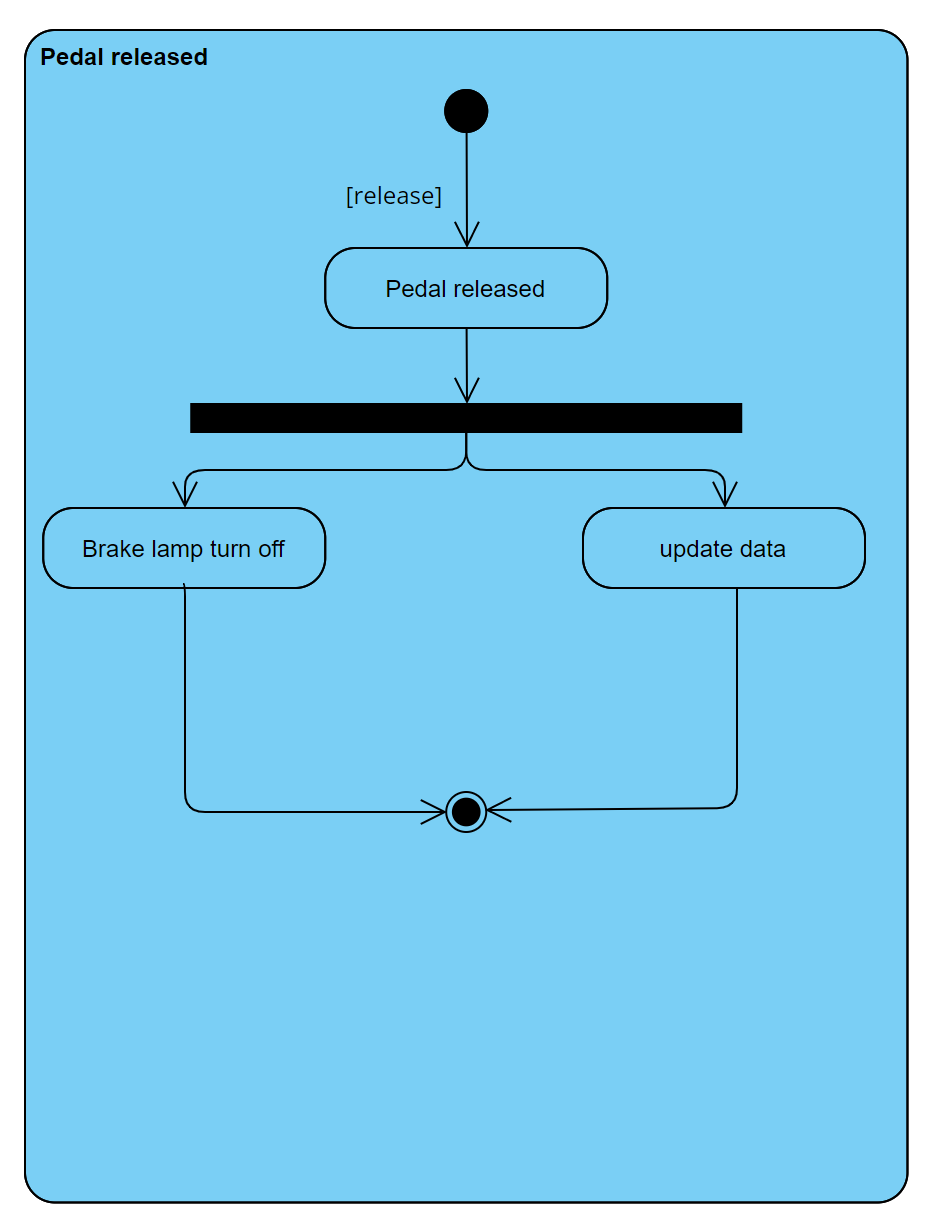
\includegraphics[width=0.3\textwidth]{AD_pedalrelease}
    \caption{Activity diagram when the pedal is released}
    \label{fig:AD_pedalrelease}
\end{figure}


\begin{figure}[h]
    \centering
    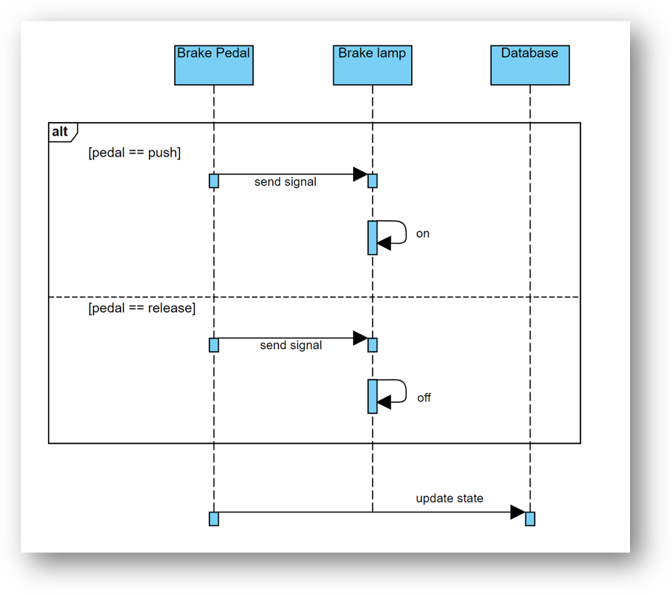
\includegraphics[width=0.5\textwidth]{sequence_diagram}
    \caption{Sequence Diagram}
    \label{fig:sequence_diagram}
\end{figure}

Eventually, by analysing all the pervious diagram,  we are able to refine our system architecture as shown in ``Fig. \ref{fig:system_architecture}".  This indicates that we are ready for implementation stage, which will be the focus of the following subsection.

\begin{figure}[h]
    \centering
    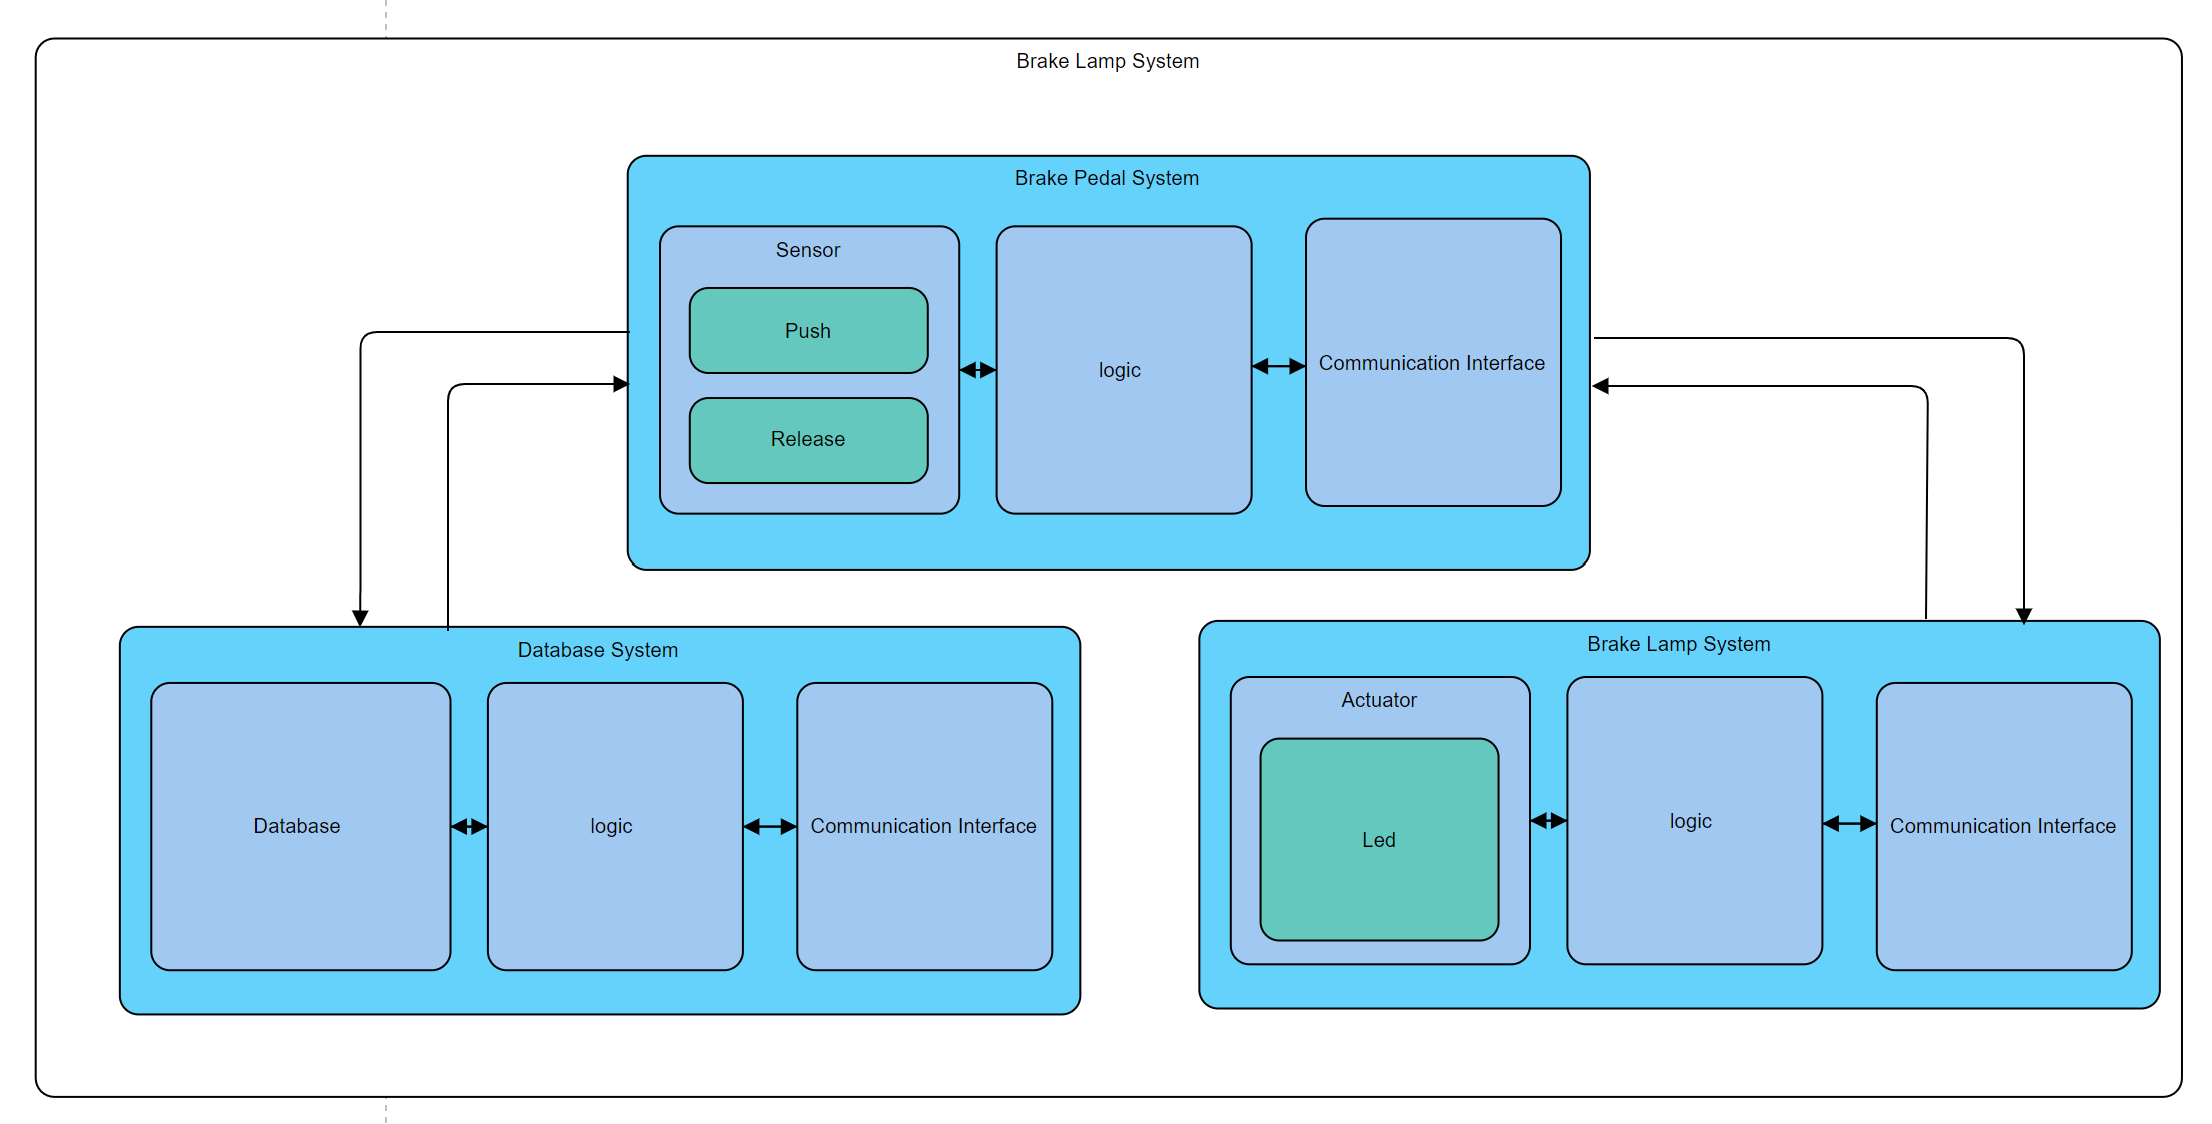
\includegraphics[width=0.6	\textwidth]{system_architecture}
    \caption{System Architecture}
    \label{fig:system_architecture}
\end{figure}

\subsection{Implementation}
For the implementation we divide it into two parts which is hardware and software part. We will first explain the hardware part followed by software part.

\subsubsection{Hardware}

For the hardware setup we will use Arduino UNO with CAN module as shown in ``Fig. \ref{fig:MCP2521}" to represent each subsystem as drawn in the system architecture that we present before in ``Fig. \ref{fig:system_architecture}" which are pedal system, database system and brake lamp system as shown in ``Fig. \ref{fig:subsystem_pedal}", ``Fig. \ref{fig:subsystem_database}", ``Fig. \ref{fig:subsystem_lamp}". The CAN module that we are used is MCP2515. For the connection with between the Arduino and the CAN module, we use SPI communication protocol. Considering that the protocol should work for long distance, we also use ca. 1.5 meter for the connection between subsystem. After we have done the setup as illustrate in Figure ``Fig. \ref{fig:hardware_setup}" we proceed to the next step which is the software implementation.

\begin{figure}[h]
    \centering
    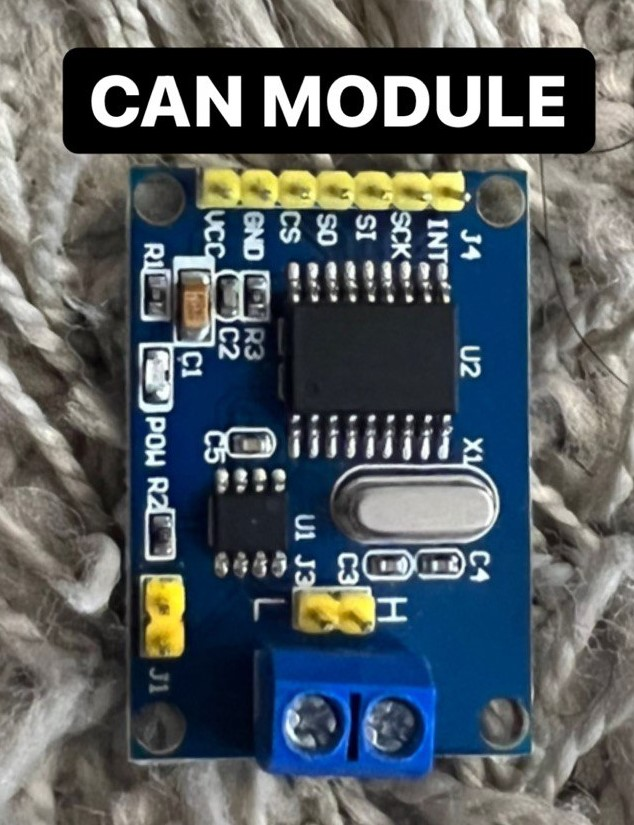
\includegraphics[width=0.15\textwidth]{MCP2521}
    \caption{MCP2521}
    \label{fig:MCP2521}
\end{figure}

\begin{figure}[h]
    \centering
    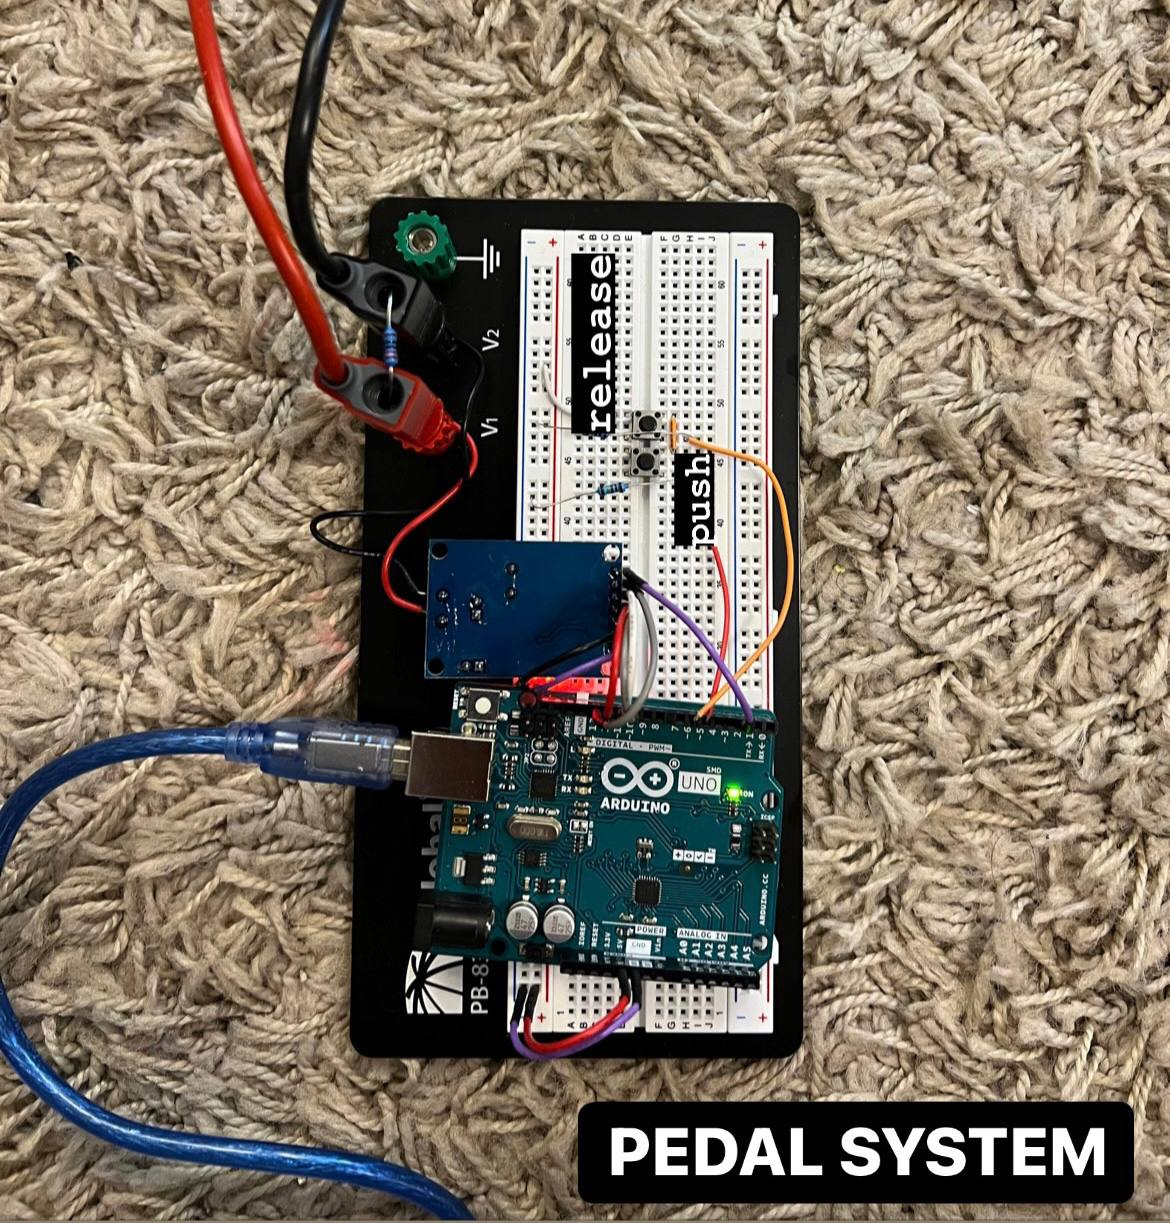
\includegraphics[width=0.3\textwidth]{subsystem_pedal}
    \caption{Pedal subsystem}
    \label{fig:subsystem_pedal}
\end{figure}
\begin{figure}[h]
    \centering
    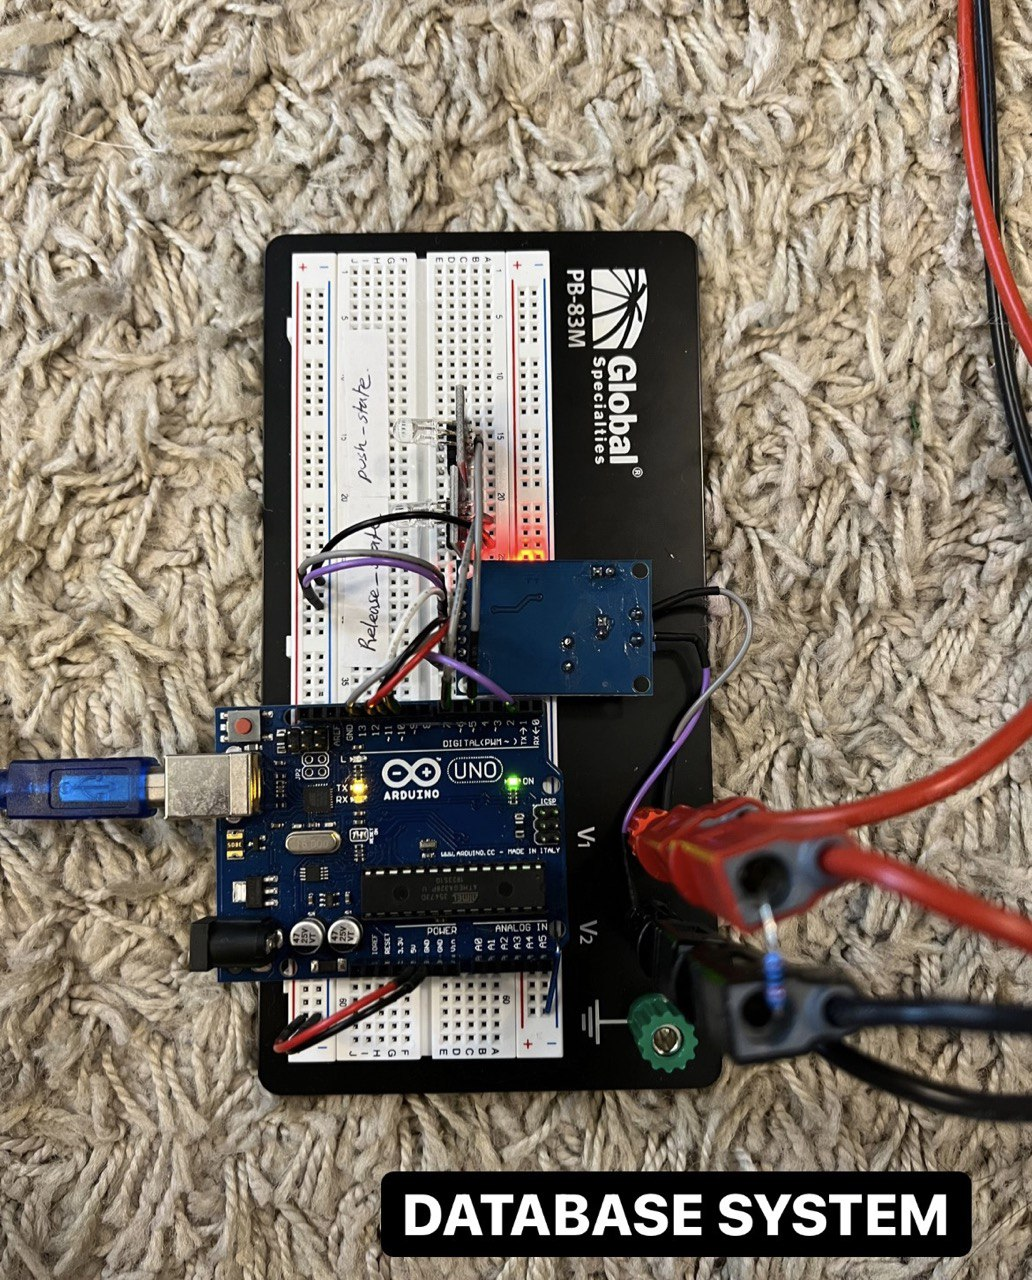
\includegraphics[width=0.3\textwidth]{subsystem_database}
    \caption{Database subsystem}
    \label{fig:subsystem_database}
\end{figure}
\begin{figure}[h]
    \centering
    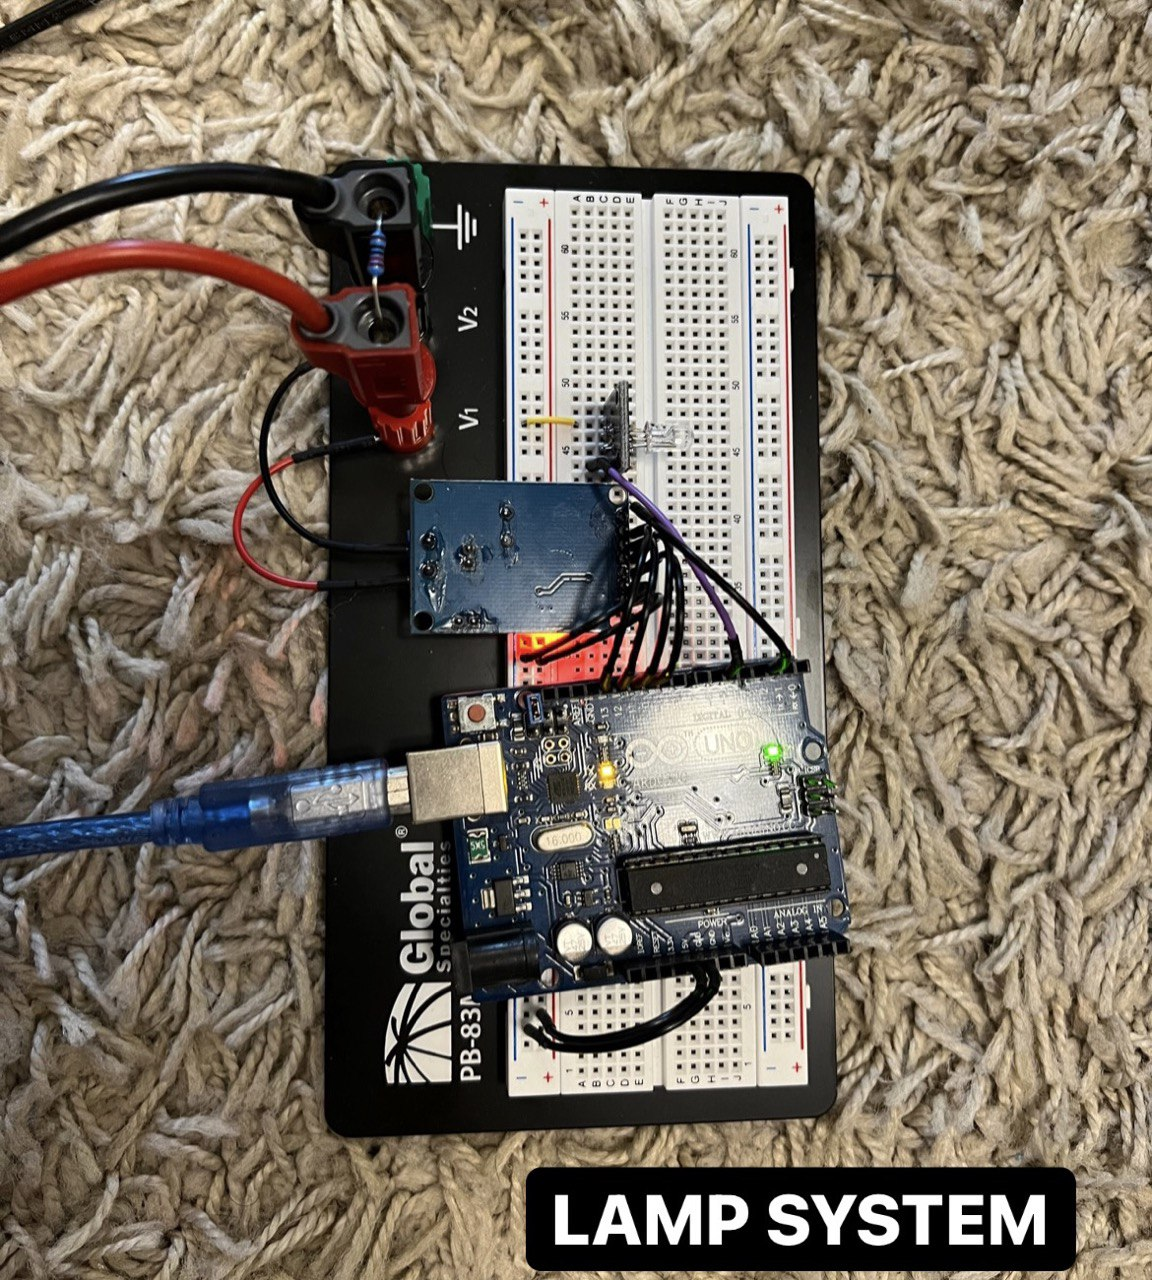
\includegraphics[width=0.3\textwidth]{subsystem_lamp}
    \caption{Brake lamp subsystem}
    \label{fig:subsystem_lamp}
\end{figure}
\begin{figure}[h]
    \centering
    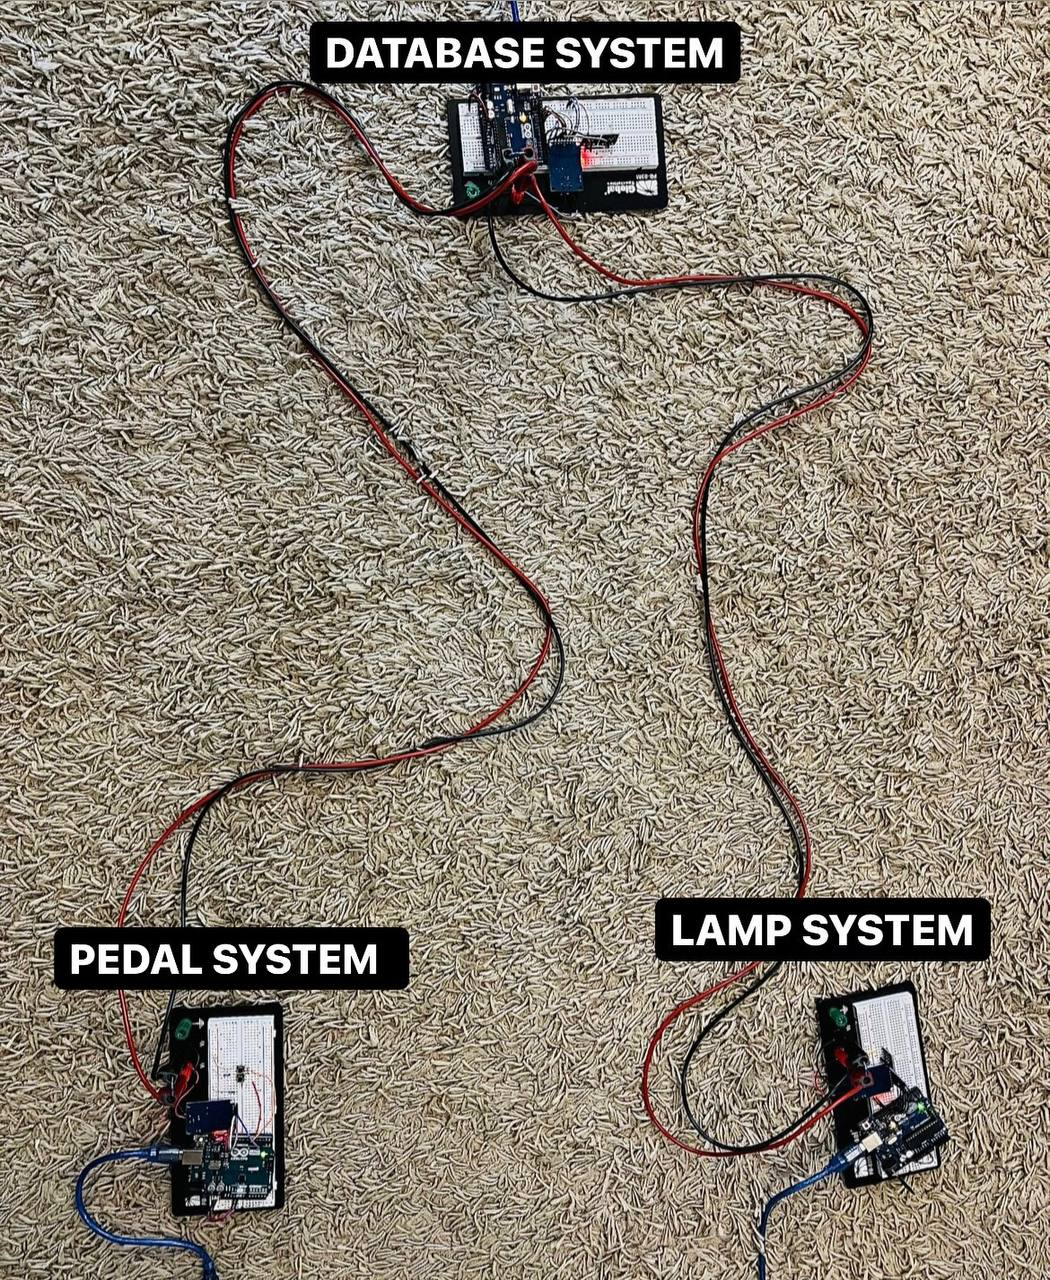
\includegraphics[width=0.3\textwidth]{hardware_setup}
    \caption{Hardware setup}
    \label{fig:hardware_setup}
\end{figure}

\subsubsection{Software}

Since we use Arduino as our subsystem platform, we use Arduino IDE to implement our software. To make the communication works as we had planned, we use CAN library provided by Arduino. In proving that It could work at high frequency, we set the data rate transfer to 1MBps. The code for each subsystem can be found in \url{https://github.com/Adib6637/Industrial-Communication}.